% !TEX root = ../thesis-example.tex
%
% Copypastas:
% "Text": \glqq Text\grqq{}
\chapter{Konzept}
\label{sec:concept}

%input	
%	tokenization
%tagging
%übergabe
%	schachtelung
%eval
%	parameter

%Goldstandards und Präzision

\begin{figure}[htb]
	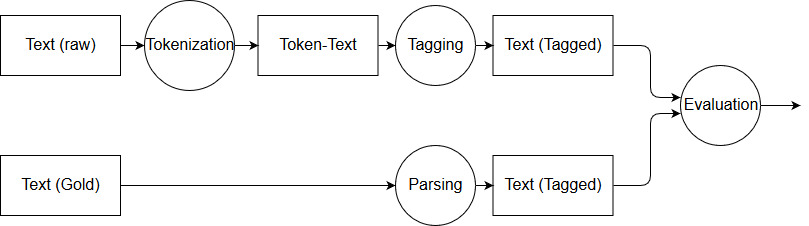
\includegraphics[width=\textwidth]{gfx/Dataflow_concept.jpg}
	\caption{Datenfluss für einen typischen Prozess von Rohdaten bis zur Evaluation}
	\label{fig:concept:overview}
\end{figure}

Aus Abbildung \ref{fig:concept:overview} können die Arbeitsschritte und Daten entnommen werden, die für Tagging und Evaluation modelliert werden müssen. Die folgenden Kapitel behandeln diese Schritte sowie insbesondere deren Eingaben und Ergebnisse.

\section{Sequenzierung}
\label{sec:concept:sequence}
Bei der Sequenzierung (\textit{Tokenization}) wird zwischen Wort- und Satzsequenzierung unterschieden \cite{Smith}. Satzsequenzierung beschäftigt sich mit einer Zerlegung des Textes in Sätze, welche für spätere Evaluation nützlich sein kann. Für Part-of-Speech-Tagging ist allerdings vorwiegend die Wort-Sequenzierung wichtig, da jedem Element der Wort-Sequenz ein Token zugewiesen wird. Außerdem sollte eine Satz-Sequenzierung vor dem Tagging nicht unbedingt stattfinden, da Tagger ggf. Kontextinformationen aus anderen Sätzen nutzen könnten, was die Auflösung von Ambiguitäten weiter unterstützen könnte. Allerdings verlangen manche Tagger eine Satzsequenzierung \cite{paroubek}.

Da Sequenzierunges-Algorithmen nicht standardisiert sind \cite{paroubek} und deren Ergebnisse von anderen - und insbesondere von Goldstandards - abweichen können, entstehen Unsicherheiten beim Vergleich dieser Sequenzen. 

\subsection{Tokenization-Unterschiede}
\label{sec:concept:sequence:tok}

Ein Token ist ein Abschnitt, zu dem ein Tag gehört, typischerweise einzelne Wörter oder Satzzeichen. Formal wird aus dem zusammenhängenden eingelesenen Wort beziehungsweise Text \textit{w} eine Menge \textit{M} von \textit{n} Teilwörtern c\textsubscript{i} 
 \[  M = \{ c_1 , c_2 , ... , c_n \} \] 
 generiert. POS-Tagger wie der von NLP4J \cite{choi} und der Stanford University \cite{Paper:StanfordTagger} können eine solche Zerlegung selbst übernehmen. Nehmen wir nun an, \textit{M} wäre die Zerlegung von \textit{w} in einem Goldstandard, und ein Tagger produziert ein Ergebnis mit der Zerlegung:
 \[  M_{tag} = \{ d_1 , d_2 , ... , d_m \} \]
Hierbei sind \textit{d\textsubscript{i}} wieder Teilworte und \textit{m} die Anzahl dieser. Spätestens wenn nun $n \neq m$ gilt, wird klar, dass \textit{M} und \textit{M\textsubscript{tag}} nicht mehr einfach iterativ verglichen werden können, da ab der Stelle \textit{p}, wo der Text unterschiedlich geteilt wurde, $ c_i \neq d_i $ sein kann, wobei $ (p \leq i \leq min\{ n, m \}) $. Es ist sogar nicht auszuschließen, dass solche Fehler bereits vorher passieren, obwohl weiterhin $n = m$ gilt.
\newline
Eines der Ziele bei der Implementierung ist also, den Vergleich von inhomogenen Token-Mengen robust gegen solche Fehler zu machen. 

\subsection{Externe Tokenization}
Um alternativ Probleme wie im vorigen Abschnitt zu verhindern, kann alternativ die Sequenzierung extern übernommen werden. D.h. dass den Taggern der Text bereits als Token-Kette übergeben wird. Hierzu muss entweder ein Tokenizer entwickelt werden, der den Taggern Tokens übergibt, die mit ihrem verlangten Format konform sind, oder im Falle eines Goldstandards kann die Token-Zerlegung aus dem annotierten Korpus selbst entnommen werden.
\\ Die meisten (alle implementierten) Tagger unterstützen das einlesen von bereits zerlegten Texten.



\section{Ergebnisformat}
\label{sec:concept:format}
Abhängig vom Tagger können Ergebnisse sehr Informationsreich sein. Der LingPipe-POS-Tagger liefert beispielsweise pro Token (Wort oder Symbol) nicht nur nicht nur das aus seiner Sicht plausibelste Tag (\textit{First-Best}), sondern auch \textit{n-1} weitere, nachstehende Optionen (\textit{N-Best}), wobei \textit{n} gewählt werden kann \cite{Lingpipedoc} . Eine solche Menge an Metainformationen kann möglicherweise von bereitgestellten Datenstrukturen seitens RapidMiner nur schwer kodiert werden. Eine speziell für Ergebnisse entworfene Datenstruktur bietet neue Freiheiten:

\paragraph{Satz-Sequenzierung} der Tag- und Token-Kette anhand von bestimmten Satzzeichen, die bei der Wort-Sequenzierung immer als eigenes Token eingefügt werden, macht robuster gegen Verschiebungen im Ergebnis wie in Abschnitt \ref{sec:concept:sequence:tok} beschrieben: Wird Satz-weise verglichen und entstehen in den Sätzen Verschiebungen durch ungleiche Token-Zerlegungen, dann verschwindet dieser Fehler, sobald ein neues Segment betreten wird, da die neuen betrachteten Segmente wieder an gleicher Stelle beginnen.
\paragraph{Anreicherung} mit Zusatzinformationen ist möglich, da im Gegensatz zu einer einfachen Textuellen Darstellung auf ein Token nicht exakt ein Tag folgen muss. Hier kann beispielsweise pro Token statt nur dem First-Best-Tag eine beliebig lange Liste der \textit{N-Best} Tags stehen.

Ein solches alternatives Format ist jedoch von Operatoren, die nicht speziell dafür vorbereitet sind (wie der Evaluationsoperator), nicht lesbar. Darum müssen Ergebnisse auch noch in einem Text-Format ausgegeben werden.

\section{Parsing von Ergebnissen}
Muss bei der Evaluation ein Text-Format angenommen werden, beispielsweise das Ergebnis in einem Goldstandard, muss entweder das angenommene Format exakt bekannt und definiert sein, oder das Dokument muss auf POS-Tags durchsucht werden. Letzteres bedeutet, dass dem Parser das Tagset des angenommenen Dokuments bekannt sein muss. Hierzu muss also jedes möglicherweise auftretende Tagset definiert werden.

\section{Evaluation}
\label{sec:concept:eval}
Um die Performance eines Taggers zu bewerten, müssen Metriken eingeführt werden. Diese entstehen aus Vergleichen zwischen annotierten Korpora und den Tagging-Ergebnissen. Im Rahmen dieses Projekts wird nur der Vergleich von Ergebnissen mit identischen Tagsets betrachtet. Abbildungsfunktionen zwischen Tagsets oder zu einem übergeordneten, generalisierten Tagset sind prinzipiell (mit einem gewissen Informationsverlust) möglich, werden aber hier außen vor gelassen. Betrachtet werden die folgenden Metriken zur Evaluation von Tagging-Ergebnissen:



\subsection{Per-Tag-Accuracy}

Die Per-Tag-Accuracy (ab hier nur \textit{Accuracy}) ist die wichtigste und einfachste Form der Bewertung eines Taggers. Sie ist definiert als \cite{Rao} :

\[ \frac{\# \: korrekter \:  Tags}{\# \: aller \:  Token} \]

\subsection{Per-Sentence-Accuracy}

Analog zur Accuracy pro Tag kann auch Accuracy pro Satz definiert werden:

\[ \frac{\# \: vollständig \: korrekter \:  Sätze}{\# \: aller \:  Sätze} \]

Hierzu müssen jedoch über Wort-Sequenzen hinaus auch Satz-Sequenzen definiert werden. Das fällt jedoch relativ leicht, da man die Sätze einfach nach jedem Satzzeichen-Token abschließen kann.

\subsection{Confusion Matrix und daraus resultierende Metriken}
Konzentrieren wir uns auf bestimmte Tags (Labels), können wir genauere Aussagen Treffen
(Für allgemeine Definitionen siehe \cite{Rao}, für mehrklassige Klassifizierungsprobleme siehe \cite{Web:rxnlp}). Zuerst bilden wir die \textit{Confusion Matrix}. In Abbildung \ref{fig:intro:pos:metrics:confusion} befindet sich ein Beispiel dafür. In dieser Matrix wird gegenübergesetzt, wie viele Labels aus dem Goldstandard als welche Labels vom Tagger vorhergesagt wurden.
\begin{description}

\item[True Positives] für Label X (kurz TP(X)) sind Vorhersagen, die dem Goldstandard entsprechen (in der Abbildung Gelb markiert).
\item[False Positives] (FP(X)) sind alle Vorhersagen X, die dem Goldstandard widersprechen.
\item[True Negatives] (TN(X)) sind alle Vorhersagen, die nicht X sind, und auch im Goldstandard nicht X lauten.
\item[False Negatives] (FN(X)) sind alle Vorhersagen, die nicht X sind, im Goldstandard aber X.
\end{description}

\begin{figure}[htb]
	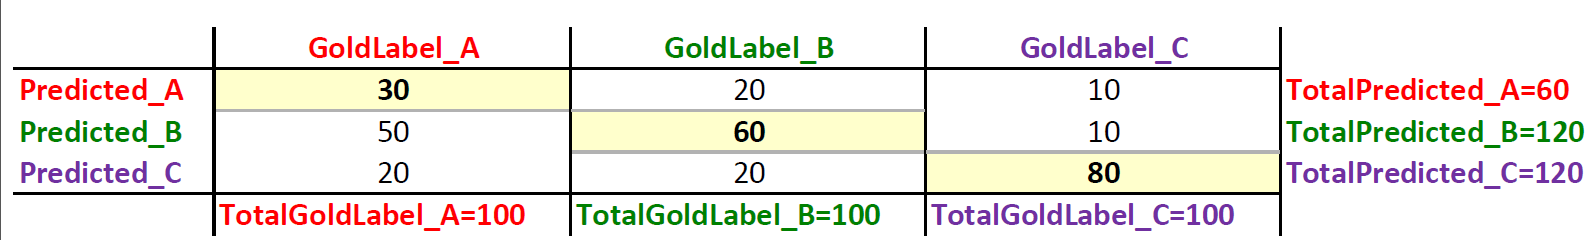
\includegraphics[width=\textwidth]{gfx/multi-class-confusionmatrix.png}
	\caption{Beispiel für eine Confusion Matrix für Labels A, B, C. Entnommen von \cite{Web:rxnlp}}
	\label{fig:intro:pos:metrics:confusion}
\end{figure}

Daraus lassen sich Precision(Wie viele der Vorhersagen X waren korrekt?), Recall(Wie viele X im Goldstandard wurden korrekt erkannt?) und der F1-Score(auch F-Score, harmonisches Mittel aus Precision und Recall) berechnen:
\[ Precision(X) \: = \: \frac{TP(X)}{TP(X)+FP(X)}\: = \: \frac{Korrekte\:X}{Vorhergesagte\:X} \]
\[ Recall(X) \: = \: \frac{TP(X)}{TP(X)+FN(X)} \: = \: \frac{Korrekte\:X}{X\:im\:Goldstandard} \]
\[ F1\mbox{-}Score \: = \: 2*\frac{Precision(X)*Recall(X)}{Precision(X)+Recall(X)} \]

Für alle drei dieser Metriken steht der Wert 1 für vollständig richtig und 0 für vollständig falsch.


\section{Zusammenfassung}
\label{sec:concept:conclusion}

In der Implementierung muss dafür gesorgt werden, dass Sequenzierungsunterschiede minimal bis gar nicht vorhanden sind, um Problemen bei der Evaluation vorzubeugen. Dies kann dadurch geschehen, dass die Sequenzierung vorweg stattfindet und den Taggern bereits sequenzierter Text übergeben wird. Es wurde festgestellt, dass zum erfolgreichen Parsen von Goldstandards und Ergebnissen die Tagsets definiert werden müssen. Zusätzlich wurde eine Datenstruktur beschrieben, mit der möglichst viele Informationen zum Tagging-Ergebnis beigelegt werden können. Letztlich wurden die Evaluationsmetriken definiert, mit denen wir die Qualität eines Ergebnisses beurteilen können.

Mit diesen Definitionen und Feststellung können wir uns nun der der tatsächlichen Planung und Implementierung der Erweiterung zuwenden.
